
\documentclass[a4paper,twoside,10pt]{article}

\usepackage{amsfonts,enumerate,bm,color,graphicx}
\input{symdef.inc}
\setlength{\textheight}{24cm}
\setlength{\textwidth}{14cm}
\setlength{\topmargin}{-1.5cm}
\setlength{\oddsidemargin}{0.5cm}
\setlength{\evensidemargin}{-0.5cm}
\pagestyle{empty}


\begin{document}

%--- CUSTOMIZATION COMMANDS ---%

\newenvironment{itmz}%
{ \vspace{-\parskip} \begin{itemize} }%
{ \end{itemize} }
\def\flux{{\cal F}_\nu}

%--- TITLE ---%

\begin{center}
  {\Large \bf
   Electromagnetism (FK4005e)\\[2mm]
   Final Examination} \\[4mm]
\end{center}
All the problem carry 20 marks.  
You can use the Student Handbook during the exam. No electronic devices are allowed
except calculators. 
\bigskip

%--- PROBLEMS ---%



\begin {enumerate}

\item Consider a sphere filled with electric charge density $\rho(r)$ that depends only
on the radial coordinate $r$. The electric charge density is given by 
\begin{equation}
\rho(r) = exp(-r)
\end{equation} 
\begin{enumerate}
\item Calculate the Electric field everywhere in space. (10 p) 
\item Calculate the energy that has been spent in assembling the sphere. (10 p) 
\end{enumerate}

\item Consider a $.303$ bullet of mass $10$ gm moving with a speed of $844 {\rm m s}^{-1}$.
If it carries a charge of $1$ Coulomb (which is never the case) and enters a region with 
a magnetic field of 1 Tesla as shown in the figure below, calculate:
\begin{enumerate}
\item The radius of the circular path the bullet takes. 
\item Sketch the path. 
\end{enumerate}
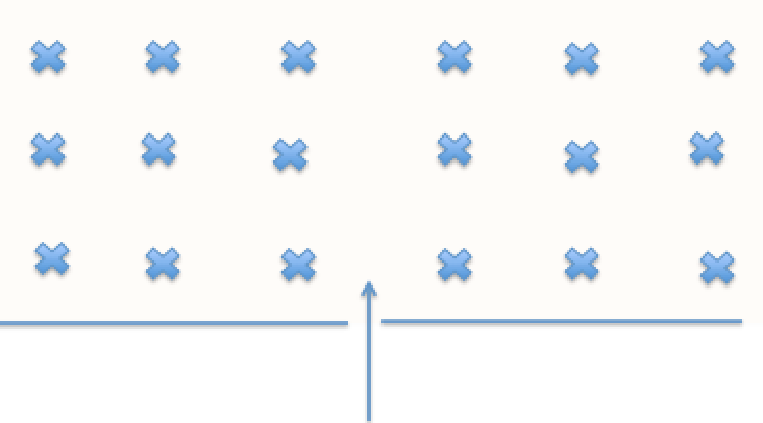
\includegraphics[width=0.90\columnwidth]{em_exam_pic1.pdf}



\item 
Start with the Maxwell's equations in free space:
\begin{eqnarray}
\dive \EE &=& \frac{\rho}{\epsilon_0} \label{eq:gauss}\\
\curl \EE &=& -\delt \BB \label{eq:faraday} \\
\dive \BB &=& 0 \label{eq:pole} \\
c^2\curl \BB &=& \frac{1}{\epsilon_0} \JJ  + \delt \EE \label{eq:ampere} 
\end{eqnarray}
Where, $\EE$ and $\BB$ are the electric and magnetic field, $\rho$ is the
volume charge density and $\JJ$ is the volume current density, $c$ is the speed of
light in vacuum and $epsilon_0$ is the permitivity of vacuum. 
Add to them the equation for charge conservation
\begin{equation}
\dive \JJ = -\delt \rho 
\label{eq:cont}
\end{equation}
Then show that: 
\begin{enumerate}
\item \Eq{eq:pole} is consistent with the divergence of \eq{eq:faraday}. 
\item \Eq{eq:cont} follows from taking divergence of \eq{eq:ampere}. 
\item Show that in empty space ($\rho=0$ and $\JJ = 0$ ) the electric
field satisfied the wave equation
\begin{equation}
\lap \EE - \frac{1}{c^2} \frac{\partial^2}{\partial t^2} \EE = 0 
\end{equation}
\end{enumerate}




\item Consider an incompressible fluid under constant gravity $g$
  acting along the negative $z$ direction.  The fluid is at rest and
its density varies as $\rho = \exp(\beta z)$ as a function of the 
vertical coordinate. Suppose further that the fluid is confined
between two rigid planes at $z=0$ and $z=d$.  At these two boundaries
$w = 0$ and $D w = 0 $ where $w$ is the vertical component of
velocity and $D \equiv d/dz$. Set up and solve the linear stability
problem. If you assume that the perturbations can be expanded as 
\begin{equation}
      \exp(ik_x x + ik_y y + nt)
\end{equation} 
the show that 
\begin{equation}
      \frac{g\beta}{n^2}  = 1 + \frac{1}{k^2 d^2} \left[ \frac{1}{4}
        \beta^2 d^2 + m^2 \pi^2 \right]
\end{equation}
where $m$ is an integer, and $k^2 = k_x^2 + k_y^2$.
From this show that the density variation is stable only if $\beta$ is
negative. (20 points)  


\end{enumerate}

\end{document}

